
\chapter{More on measures}
In this chapter we discuss vector-valeud measures and the relationships between measured spaces.
These turn out to be especially useful in applications, including probability theory, so we introduce the languages of probability theory and ergodic theory in this chapter as well.

\section{Measurable maps}
In topology, a continuous map is one that pulls back open sets to open sets.
Here we have no open sets to work with --- only measurable spaces --- but this turns out to be exactly what we want.

\begin{definition}
Let $(X, \Sigma)$ and $(Y, \Gamma)$ be measurable spaces.
A \dfn{measurable map} $f: X \to Y$ is a map such that for every measurable set $A \in \Gamma$, $f^{-1}(A)$ is measurable.

A \dfn{measurable isomorphism} is a measurable map $f: X \to Y$ such that $f$ is a bijection and $f^{-1}$ is measurable.
If a measurable isomorphism exists, we say that $X,Y$ are \dfn{isomorphic} as measurable spaces, or that $\Sigma$ and $\Gamma$ are \dfn{isomorphic} as $\sigma$-algebras.
\end{definition}

\begin{example}
Isomorphism of measurable spaces is a very weak notion.
If $X$ is an uncountable \dfn{Polish space} --- a complete separate metric space --- then we call its Borel $\sigma$-algebra $\Sigma$ the \dfn{standard Borel algebra}.
A theorem of a branch of logic known as descriptive set theory implies that there is only one standard Borel algebra, up to isomorphism.
So any two Polish spaces, when viewed as measurable spaces, are the same!
\end{example}

\begin{definition}
Let $(X, \Sigma, \mu)$ be a measured space, $(Y, \Gamma)$ a measurable space, and $f: X \to Y$ a measurable map.
We define $f_{*}(\mu)$ on $(Y, \Gamma)$ by
\[f_{*}(\mu)(E) = \mu(f^{-1}(E))\]
and call $f_{*}(\mu)$ the \dfn{pushforward measure} of $\mu$ by $f$.
\end{definition}

\begin{example}\label{lebesgue measure torus}
Let $\Torus$ be the circle, viewed for now as the set $\{z \in \CC: |z| = 1\}$.
Then $\Torus$ has its Borel $\sigma$-algebra $\Gamma$.
Let $\Sigma$ be the Borel $\Sigma$-algebra of $\RR$ and $\mu$ the Lebesgue measure restricted to $\Sigma$.
Then we have a continuous map $f: [0, 1] \to \Torus$ defined by
\[f(x) = e^{2\pi ix}.\]
Every continuous map between Borel measurable spaces is measurable, so $f$ is.
The pushforward measure $\nu = f_{*}(\mu)$ is known as the \dfn{Lebesgue measure} on $\Torus$.
The diligent reader will check that $\nu$ agrees with the notion of arc length defined in multivariable calculus (Exercise~\ref{arc length exercise}).
\end{example}

\begin{definition}
Let $(X, \mu)$ and $(Y, \nu)$ be measured spaces.
A \dfn{measure-preserving map} is a measurable map $f: X \to Y$ such that
\[\nu = f_{*}(\mu).\]
If $f$ is a measurable isomorphism, we call $f$ a \dfn{measure-preserving isomorphism}.
\end{definition}

\begin{definition}
Let $X$ be a set, $(Y, \Gamma)$ a measurable space, and $F: X \to Y$ a map.
The \dfn{pullback $\sigma$-algebra} $F^{*}\Gamma$ is the $\sigma$-algebra of sets of the form $F^{-1}(A)$ where $A \in \Gamma$.
\end{definition}

\begin{subsec}
We need to check that the definition of a pullback $\sigma$-algebra makes sense.
Namely, we must show that if $F: X \to Y$ is a map, and $\Gamma$ a $\sigma$-algebra on $Y$, then $F^{*}\Gamma$ is a $\sigma$-algebra.
This is part of the content of Exercise~\ref{pullback makes sense}, which also shows that $F^{*}\Gamma$ is the smallest $\sigma$-algebra for which $F$ is measurable.
\end{subsec}

\begin{exercise}
Show that measurable spaces with measurable maps form a category.
\end{exercise}

\begin{exercise}\label{arc length exercise}
By an \dfn{arc} we mean a compact connected subset of $\Torus$.
Recall the definition of the length of an arc from calculus.
Show that the length of an arc equals its Lebesgue measure.
\end{exercise}

%\begin{exercise}\label{Lebesgue measure on sphere}
%Let $S^{d}$ denote the unit sphere in $\RR^{d+1}$, and let $N$ be its open northern hemisphere.
%Let $U$ be the open unit ball in $\RR^{d}$, so $U \times \{0\}$ is a subset of the unit ball of $\RR^{d+1}$.
%Show that the map $p: N \to \RR^{d+1}$, $p(x_{1}, \dots, x_{d+1}) = (x_{1}, \dots, x_{d}, 0)$, is a homeomorphism between $N$ and $U \times \{0\}$.
%So the pushforward of Lebesgue measure on $\RR^{d}$ by $p^{-1}$ gives a Borel measure on $N$, which we call \dfn{Lebesgue measure} on $N$.
%Use this fact to define Lebesgue measure of any Borel subset of $S^{d}$.
%Show that when $d = 2$, Lebesgue measure on $S^{d}$ agrees with the usual notion of surface area, up to a constant factor.
%\end{exercise}
% I think this exercise is just wrong !

\begin{exercise}\label{pullback makes sense}
Let $F: X \to Y$ be a map, $\Gamma$ a $\sigma$-algebra on $Y$.
Show that $F^{*}\Gamma$ is a $\sigma$-algebra on $X$ and $F: (X, F^{*}\Gamma) \to (Y, \Gamma)$ is measurable.
Conversely, show that $F^{*}\Gamma$ is the intersection of all $\sigma$-algebras $\Sigma$ on $X$ such that $F: (X, \Sigma) \to (Y, \Gamma)$ is measurable.
\end{exercise}

\section{Hausdorff measures}
At this point we have defined Stieltjes measures.
In particular, we defined the Lebesgue measure and the Dirac measure.
Let us treat some more measures.

TODO:\@ Hausdorff measures


\begin{example}\label{Lebesgue measure on sphere}
An important example of Hausdorff measure is the $d-1$-dimensional Hausdorff measure in $\RR^{d}$.
When restricted to the unit sphere
\[S^{d - 1} = \{x \in \RR^{d}: |x| = 1\},\]
and normalized so that the total measure of the sphere is $1$, the Hausdorff measure is called the \dfn{spherical Lebesgue measure}, denoted $\sigma_{d - 1}$.
The spherical Lebesgue measure is especially important because, once integration has been defined, we will have
\[\int_{\RR^{d}} f(x) ~dx = \int_{0}^{\infty} \int_{S^{d - 1}} f(r\omega) r^{d - 1}~d\sigma_{d - 1}(\omega) ~dr,\]
which is a generalization of the classical formula
\[\int_{-\infty}^{\infty} \int_{-\infty}^{\infty} f(x, y) ~dx ~dy = \int_{0}^{\infty} \int_{0}^{2\pi} f(r \cos \theta, r \sin \theta) r~d\theta ~dr\]
for integration in polar coordinates. Here $r^{d - 1} d\sigma_{d - 1}(\omega)$ plays the role of $r~d\theta$.
\end{example}



\section{Measures on compact matrix groups}


\section{Vector-valued measures}
Recall that by definition, a measure $\mu$ is a $\sigma$-additive function $\mu: \Sigma \to (-\infty, \infty]$, where $\Sigma$ is a $\sigma$-algebra.
However, the definition of $\sigma$-additive function makes sense even if $(-\infty, \infty]$ is replaced by a more general codomain, and we will have use for this when we integrate functions in more general codomains than the real numbers.

\begin{subsec}
Let $B$ be a Banach space, as discussed in Appendix~\ref{Banach space appendix}.
If the reader is unfamiliar with Banach spaces, they can take $B = \CC^{d}$ and not lose any insight.
If $(x_{n})$ is a sequence in $B$, then (\ref{banach space series}) is the definition of the infinite sum $\sum_{n} x_{n}$.
\end{subsec}

\begin{definition}
Let $\Sigma$ be a $\sigma$-ring and $B$ a Banach space.
A \dfn{vector-valued measure} on $\Sigma$, or simply a \dfn{measure}, is a function $\mu: \Sigma \to B$ such that whenever $(E_{n})$ are countably many disjoint sets in $\Sigma$,
\[\mu\left(\bigcup_{n} E_{n}\right) = \sum_{n} \mu(E_{n}).\]
\end{definition}

\begin{example}
The most important examples of vector-valued measures will be of the following form.
Let $\nu$ be a positive measure on a measurable space $X$, and let $f: X \to B$ be an ``integrable function''.
We will get back to what this means later --- but, taking the definition of integration as a black box, set
\[\mu(E) = \int_{E} f(x) ~d\nu(x).\]
Then $\mu$ is a vector-valued measure, and its ``derivative'' is $f$.
This will be the setting in which we generalize the fundamental theorem of calculus.
\end{example}

\begin{subsec}
Frequently, positive measures are easier to work with than vector-valued measures, so we will mainly spend this section developing tools to convert problems about vector-valued measures into problems about positive measures.
\end{subsec}

\begin{definition}
Let $\mu$ be a measure. The \dfn{total variation measure} $|\mu|$ of $\mu$ is defined by
\[|\mu|(E) = \sup_{E_{1}, \dots, E_{n}} \sum_{i=1}^{n} ||\mu(E_{i})||_{B}\]
where the supremum ranges over finite sequences $E_{1}, \dots, E_{n}$ of disjoint measurable sets such that $E = \bigcup_{i} E_{i}$.
\end{definition}

\begin{theorem}
Every total variation measure is a positive measure.
\end{theorem}
\begin{proof}
Let $\mu$ be a measure. Then $|\mu|$ is nonnegative. If $E \subseteq F$ are measurable sets, write $F = E \cup (F \setminus E)$ to see that $|\mu|(E) \leq |\mu|(F)$.

To see that $|\mu|$ is $\sigma$-additive, suppose that $F,G$ are disjoint measurable sets, $E = F \cup G$.
Write $F = \bigcup_{i \leq m} F_{i}$ and $G = \bigcup_{j \leq n} G_{j}$ where the $F_{i},G_{j}$ are all disjoint; then
\[|\mu|(E) \geq \sum_{i=1}^{m} ||\mu(F_{i})||_{B} + \sum_{j=1}^{n} ||\mu(G_{j})||_{B}.\]
Thus $|\mu|(E) \geq |\mu|(F) + |\mu|(G)$, so by induction if $E = \bigcup_{i \leq m} E_{i}$ where the $E_{i}$ are disjoint, then $|\mu|(E) \geq \sum_{i \leq m} |\mu|(E_{i})$.
Using the monotonicity, it follows that if $(E_{i})$ is a disjoint countable sequence of sets and $E = \bigcup_{i} E_{i}$, then
\[|\mu|(E) \geq \sum_{i=1}^{\infty} |\mu|(E_{i}).\]

Conversely, suppose that $E = \bigcup_{j} E_{j} = \bigcup_{i\leq n} F_{i}$ where $(E_{j})$ is a disjoint countable sequence and $(F_{i})$ is a disjoint finite sequence. Then
\begin{align*}
\sum_{i=1}^{n} ||\mu(F_{i})||_{B} &= \sum_{i=1}^{n} \left|\left|\mu\left(\bigcup_{j=1}^{\infty} \left(F_{i} \cap E_{j}\right)\right)\right|\right|_{B} \leq \sum_{i=1}^{n} \sum_{j=1}^{\infty} ||\mu(F_{i} \cap E_{j})||_{B} \\
&= \sum_{j=1}^{\infty} \sum_{i=1}^{n} ||\mu(F_{i} \cap E_{j})||_{B} \leq \sum_{j=1}^{\infty} |\mu|(E_{j}).
\end{align*}
Here we used the fact that $E_{j} = \bigcup_{i \leq n} F_{i} \cap E_{j}$. It follows that $|\mu|(E) \leq \sum_{i=1}^{\infty} |\mu|(E_{i})$.
\end{proof}

\begin{theorem}[triangle inequality and reverse triangle inequality]\label{reverse triangle inequality}
Let $\mu,\nu$ be measures on $\Sigma$ with values in $B$. Then $|\mu + \nu| \leq |\mu| + |\nu|$ and
\[||\mu|(E) - |\nu|(E)| \leq |\mu - \nu|(E).\]
\end{theorem}
\begin{proof}
If $E = \bigcup_{i \leq n} E_{i}$, the $E_{i}$ disjoint, then
\[\sum_{i=1}^{n} ||(\mu + \nu)(E_{i})||_{B} \leq \sum_{i=1}^{n} ||\mu(E_{i})||_{B} + ||\nu(E_{i})||_{B} \leq |\mu|(E) + |\nu|(E)\]
which implies the two desired inequalities.
\end{proof}

\begin{subsec}
Let $\mu$ be a vector-valued measure.
The total variation measure $|\mu|$ can be viewed as the positive measure that ``best dominates'' $||\mu||_{B}$ in the sense that for every measurable set $E$, $|\mu(E)| \geq ||\mu(E)||_{B}$.
On the other hand, if $\mu$ is already a positive measure, then the definition of the total variation measure $|\mu|$ still makes sense, and additivity of $\mu$ implies that $\mu = |\mu|$.
Thus we can use total variation to extend definitions of measures to this more general setting.
\end{subsec}

\begin{definition}
A vector-valued measure $\mu$ is \dfn{$\sigma$-finite} if $|\mu|$ is $\sigma$-finite.
A set $E$ is \dfn{$\mu$-null} if $E$ is $|\mu|(E)$-null.
The measure $\mu$ is a \dfn{complete measure} if every $\mu$-null set is complete.
The \dfn{completion} of $\mu$ is the vector-valued measure obtained by extending the domain of $\mu$ to contain all $\mu$-null sets.
\end{definition}

\begin{exercise}
Show that the completion of a vector-valued measure is well-defined.
That is, if $(X, \Gamma)$ is a measurable space and $\mu$ is a vector-valued measure on $\Gamma$, then show that there is a $\sigma$-algebra $\Sigma$ on $X$ which contains every measurable set and every $\mu$-null set, such that $(X, \Sigma, \mu)$ is a complete measured space.
\end{exercise}

\begin{exercise}
Give an example of a vector-valued measured space $(X, \mu)$ such that $\mu(X) = 0$, but $|\mu|$ is not identically zero.
Thus, explain why we cannot define a $\mu$-null set to simply be a set $E$ such that $\mu(E) = 0$.
\end{exercise}


\section{Probability}
In 1933, Andrey Kolmogorov put probability theory --- which was long viewed as not part of rigorous mathematics --- on a sound footing by establishing three axioms that probability theory ought to satisfy.
These axioms, however, are exactly the definition of a probability measure!
Thus measure theory is an invaluable tool in applied mathematics, such as statistics.
However, even the myopic reader who only cares about pure, abstract mathematics will find probability useful to their work.

In this section we do little more than develop a language, but in later sections we will find a great use for it.

\begin{definition}
A \dfn{probability space} $(\Omega, \Sigma, P)$ is a measure space with $P(\Omega) = 1$.
Elements of $\Sigma$ are called \dfn{events} and elements of $X$ are called \dfn{outcomes}.
The quantity $P(A)$, where $A$ is an event, is called the \dfn{probability} that $A$ is true.
\end{definition}

\begin{subsec}
The intuition here is that the events form an algebra $\Sigma$ of statements that could be true or false about the world, with varying probabilities.
By an algebra of statements, more precisely, one means that it is meaningful to conjoin them using grammar: $A \cup B$ is the event that $A$ happens or $B$ happens, while $A \cap B$ is the probability that both $A$ happens and $B$ happens. The event $\Omega \setminus A$ is the probability that $A$ does not happen, and so on.
The event $\Omega$ is vacuously true; it represents the statement ``$2 + 2 = 4$''.
The event $\emptyset$, on the other hand, is vacuously false; it represents the statement ``$2 + 2 = 5$''.
Thus probability theory sits somewhere between analysis and logic in the world of mathematics, and the language used in the following definition is motivated.
\end{subsec}

\begin{definition}
Let $(\Omega, \Sigma, P)$ be a probability space.

The event $A \cup B$ is called $A$ \dfn{or} $B$, or the \dfn{disjunction} of $A,B$, and the event $A \cap B$ is called $A$ \dfn{and} $B$, or the \dfn{conjunction} of $A,B$.
The event $\Omega \setminus A$ is called \dfn{not} $A$, or the \dfn{negation} of $A$.

The event $\Omega$ is said to be \dfn{true}, and the negation $\emptyset$ of true is said to be \dfn{false}.
An event $A$ is said to be \dfn{almost surely true} if $P(A) = 1$, and \dfn{almost surely false} if $P(A) = 0$.

A set $\Sigma_{0} \subseteq \Sigma$ of events is said to be \dfn{mutually exclusive} if for every $A, B \in \Sigma_{0}$, $A \cap B$ is almost surely false.
\end{definition}

\begin{subsec}
The $\sigma$-additivity of the measure $P$ says that if a countable set $\Sigma_{0}$ of events is mutually exclusive, its disjunction $A$ satisfies
\[P(A) = \sum_{B \in \Sigma_{0}} P(B),\]
thus for example we have the \dfn{inclusion-exclusion formula}
\[P(E \cup F) = P(E) + P(F) - P(E \cup F)\]
valid for any two events $E,F$ familiar from elementary probability theory.
\end{subsec}

\begin{subsec}
So far we have only discussed events. But what role do outcomes play?
Outcomes are ``microstates'' and each outcome carries all possible information about a particular state that the universe could be --- the position and momentum of every last molecule, the value of every card in every player's hand.
But we are just puny mortal observers of the universe; we cannot possibly have access to all that information!
So outcomes are not terribly useful, and one generally avoids ever mentioning outcomes directly.
What we mortal observers can observe are random variables.
\end{subsec}

\begin{definition}
Let $(\Omega, P)$ be a probability space and $E$ be a measurable space.
A \dfn{random variable} of \dfn{type} $E$, also known as an \dfn{observable} of type $E$, is a measurable map $\Omega \to E$.
\end{definition}

\begin{subsec}
The points of the space $E$ represent possible values that an experiment can return.
The random variable $X: \Omega \to E$ represents an experiment. If $\omega$ is an outcome, $X(\omega)$ is the result of the experiment $X$ if the universe is in state $\omega$.
One generally takes $E = \RR$ with its Borel $\sigma$-algebra, since most experiments return numerical data, but there are other examples of useful types $E$; for example, points of $E$ are often sequences, vectors, or graphs.
If the type of $X$ is clear --- especially if it is $\RR$ --- we will suppress it.
\end{subsec}

\begin{subsec}
Let $X$ be a random variable (of type $\RR$).
The sets $[x, \infty)$ are Borel, so the sets $\{X \geq x\} = \{\omega \in \Omega: X(\omega) \geq x\}$ are actually events.
The probability of the event $\{X \geq x\}$ is frequently of interest, so we make the following definition.
\end{subsec}

\begin{definition}
Let $X$ be a random variable of type $E$.
The \dfn{distribution} $\mu_{X}$ of $X$ is the pushforward $X_{*}P$ of $P$ on $E$.
If $Y$ is another random variable and $\mu_{X} = \mu_{Y}$, we say that $X,Y$ are \dfn{identically distributed}.
\end{definition}

\begin{subsec}
Unraveling the definitions, if $A \subseteq E$ is a measurable set,
\[\mu_{X}(A) = P(X \in A) = P(\{\omega \in \Omega: X(\omega) \in A\}).\]
For example, if $E = \RR$ then $\mu_{X}([x, \infty))$ is the probability that $X \geq x$.
We think of two identically distributed random variables as being isomorphic, but not the same.
\end{subsec}

\begin{figure}
\label{bell curve figure}
\caption{A Gaussian cdf (in blue) and its derivative, the familiar ``bell curve" from elementary statistics (in green).}
\centering 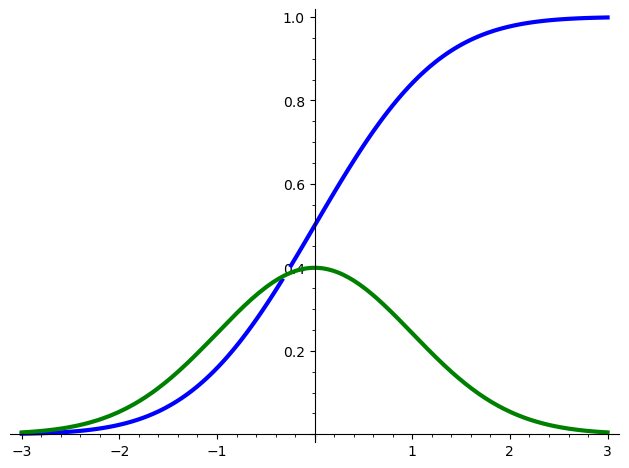
\includegraphics[width=0.5\textwidth]{graphics/bell_curve}
\end{figure}

\begin{example}
\label{Gaussian CDF}
An especially important and familiar distribution is the \dfn{Gaussian measure} $N(0, 1)$ on $\RR$, which is the Stieltjes measure defined by the \dfn{Gaussian cumulative distribution function} (or \dfn{Gaussian cdf})
\[f(x) = \frac{1}{\sqrt{2\pi}} \int_{-\infty}^{x} \exp\left(-\frac{y^{2}}{2}\right) ~dy.\]
In other words, the measure of $[\alpha, \beta)$ is by definition $f(\beta) - f(\alpha)$.
Here the factor of $1/\sqrt{2\pi}$ is to ensure that $N(0, 1)$ is actually a probability measure, c.f. Example~\ref{Gaussian integral formula}.
A random variable with distribution $N(0, 1)$ is said to be a \dfn{standard-normally distributed} random variable. More generally, one defines $N(\mu, \sigma^{2})$ to be the Stieltjes measure defined by the cumulative distribution function
\[x \mapsto \frac{1}{\sigma\sqrt{2\pi}} \int_{-\infty}^{x} \exp\left(-\frac{1}{2}{\left(\frac{y - \mu}{\sigma}\right)}^{2}\right) ~dy,\]
and a random variable with distribution $N(\mu, \sigma^{2})$ is said to be \dfn{normally distributed} with mean $\mu$ and standard deviation $\sigma$.
See Figure \ref{bell curve figure}.
\end{example}

\begin{subsec}
Recall that in elementary probability theory two events $A,B$ are said to be independent if $P(A) = P(A|B)$, where $P(A|B)$ (``the probability of $A$ given $B$'') is by definition $P(A \cap B)/P(B)$.
The intuition is that if we know that $B$ is true, then we want to restrict to subsets of $B$ and rescale the probability measure $P$ so that $B$ is almost surely true.
However, if $A$ and $B$ really have nothing to do with each other, the probability of $A$ given $B$ is just the probability of $A$.
We can write this in a more symmetrical form, which also avoids the issue of division by zero, as in the following definition.
\end{subsec}

\begin{definition}
Let $(\Omega, \Sigma, P)$ be a probability space and $(E, \Gamma)$ a measurable space.

Countably many events $A_{n} \in \Sigma$ are said to be \dfn{independent} if
\[P\left(\bigcap_{n} A_{n}\right) = \prod_{n} P(A_{n}).\]
Countably many $\sigma$-algebras $\mathcal A_{n} \subseteq \Sigma$ are said to be \dfn{independent} if for every $A_{n} \in \mathcal A_{n}$, the events $A_{n}$ are independent.
Countably many random variables $X_{n}$ of type $E$ are said to be \dfn{independent} if the pullback $\sigma$-algebras $X_{n}^{*}\Gamma$ are independent.

Random variables $X,Y$ are said to be \dfn{iid} if they are independent and identically distributed.
\end{definition}

\begin{subsec}
The idea in the definition of independent random variables is that the pullback $\sigma$-algebra $X^{*}\Gamma$ is the set of events that can be checked as true or false by measuring $X$.
\end{subsec}

\begin{example}
Suppose that I am playing a game of cards.
Every time I draw a card, I put it back in the deck and then shuffle again.
Let $X_{n}$ be $1$ if I draw the queen of hearts on turn $n$, and $0$ otherwise.
Then the distribution of $X_{n}$ is $(51/52)\delta_{0} + (1/52)\delta_{1}$, where $\delta_{x}$ is the Dirac measure at $x$.
Since I shuffle between turns, the $X_{n}$ are independent.
So the $X_{n}$ are iid.
\end{example}

\begin{exercise}
Verify the inclusion-exclusion formula
\[P\left(\bigcup_{i=1}^{n} A_{i}\right) = \sum_{k=1}^{n} {(-1)}^{k+1} \sum{1 \leq i_{1} < \cdots < i_{k} \leq n} P\left(\bigcap_{j=1}^{k} A_{i_{j}}\right)\]
valid for any events $A_{1}, \dots, A_{n}$.
\end{exercise}

\begin{exercise}[Skohorod representation]\label{Skohorod representation}
Let $\mu$ be a Borel probability measure on $\RR$.
Show that there is a probability space $\Omega$ and a random variable $X: \Omega \to \RR$ of distribution $\mu$.
\end{exercise}

\begin{exercise}
Let $X_{n}$ be random variables and suppose that for every $x \in \RR$, the events $X_{n} \geq x$ are independent.
Show that the $X_{n}$ are independent random variables.
\end{exercise}

\begin{exercise}
Let $X_{n}$ be independent random variables of type $E$.
Suppose that $f_{n}: E \to E$ are measurable maps.
Show that the $f_{n}(X_{n})$ are still independent.
\end{exercise}

\begin{exercise}
Let $X, Y: \Omega \to E$ be random variables.
A \dfn{morphism of random variables} $X \to Y$ is a measure-preserving map $F: \Omega \to \Omega$ such that $Y \circ F = X$.
Two morphisms $F,G$ are \dfn{equal almost surely} if $P(F = G) = 1$.
Two random variables $X,Y$ are \dfn{isomorphic} if there are morphisms $F: X \to Y$ and $G: Y \to X$ such that $F \circ G$ and $G \circ F$ are the identity almost surely (so $G$ is almost surely the inverse of $F$).

Show that being equal almost surely is an equivalence relation on the set of morphisms of random variables.
Show that random variables $\Omega \to E$ and morphisms between them, modulo the equivalence relation of being equal almost surely, form a category.
Show that two random variables are isomorphic iff they are identically distributed.
\end{exercise}

\section{Ergodic systems}
This section is used nowhere else in this book, except in some exercises; it is meant to showcase an application.

Measure-preserving maps from a measured space to itself are important in probability and thermodynamics; their study is known as \dfn{ergodic theory}.

\begin{definition}
A \dfn{measure-preserving system} $(X, \Sigma, P, f)$ consists of a probability space $(X, \Sigma, P)$ and a measure-preserving map $f: X \to X$.
\end{definition}

\begin{subsec}
We may suppress $X$ or $\Sigma$ from the notation when they are clear or unhelpful to specify.
\end{subsec}

\begin{subsec}
The intuition for measure-preserving systems is as follows.
We have a probability space $X$ whose events $A$ are properties that the world could have, and the probability $P(A)$ is the probability that the world is in that state.
The map $f$ represents the passing of time; each application of $f$ represents the passing of a unit of time.
However, the probability that the universe has property $A$ is the same today as it is tomorrow.
\end{subsec}

\begin{definition}
An \dfn{ergodic system} is a measure-preserving system $(X, \Sigma, P, f)$ for which, whenever $f(A) \subseteq A$ and $A \in \Sigma$, then $P(A) = 0$ or $P(A) = 1$.
\end{definition}

\begin{subsec}
Ergodic systems are the most important examples of measure-preserving systems.
The reason is that ergodic systems behave ``randomly''.
In an ergodic system, the universe might have property $A$ today, but this is no evidence that the universe will have property $A$ tomorrow, because every day all the properties that the universe could have get completely mixed up every time $f$ is applied.

Let $(X, P, f)$ be an ergodic system.
Imagine that $X$ is an egg; then $P$ represents picking a random point inside the egg, and $f$ represents the action of scrambling the egg, say with chopsticks.
Though $X$ is initially in an orderly state, the ergodicity of the system means that all this order is lost and all the points of $X$ get mixed up.
This is illustrated mathematically by the following example.
\end{subsec}

\begin{example}
One ergodic system is known as the \dfn{irrational rotation}.
Let $\theta \in [0, 2\pi]$ and suppose that $\theta/\pi$ is irrational.
Then the map $f(z) = e^{i\theta}z$ on the circle $\Torus$, which rotates the circle by $\theta$, defines an ergodic system $(\Torus, \mu, f)$, where $\mu$ is Lebesgue measure.
The reader who is familiar with some Fourier analysis may show this in Exercise~\ref{irrational rotation exercise}.
\end{example}

\begin{subsec}
As a sample of the power of ergodic theory, let us prove the following theorem that ``breaks the laws of thermodynamics''.
If $(X, f)$ is a measure-preserving system and $x \in X$, we let $f^{n}(x)$ denote $f \circ \cdots \circ f$, where there are $n$ copies of $f$.
The theorem is due to Carathéodory, which is naturally why it is named after Poincar\'e.
\end{subsec}

\begin{theorem}[Poincar\'e recurrence]
Let $(X, \Sigma, P, f)$ be a measure-preserving system.
For every $A \in \Sigma$, define $A^{\flat} = \{x \in A: \forall n~f^{n}(x) \notin A\}$.
Then $P(A^{\flat}) = 0$.
\end{theorem}
\begin{proof}
We first note that
\[A^{\flat} = A \setminus \bigcup_{n \in \NN} f^{n}(A)\]
which is measurable since each of the $f^{n}(A)$ are.

If $m > n$, then $f^{n}(A^{\flat}) \cap f^{m}(A^{\flat})$ is empty: if $x \in f^{m}(A^{\flat})$, so that $f^{-m}(x) \in A^{\flat}$, then by definition of $A^{\flat}$,
\[f^{-n}(x) = f^{m-n}(f^{-m}(x)) \notin A.\]

Therefore, for any $N \in \NN$,
\[P(A^{\flat}) = \frac{1}{N} \sum_{n=1}^{N} P(f^{m}(A^{\flat})) = \frac{1}{N} P\left(\bigcup_{n=1}^{N} f^{m}(A^{\flat})\right) \leq \frac{1}{N} P(X) = \frac{1}{N}.\]
So $P(A^{\flat}) = 0$.
\end{proof}

\begin{subsec}
Let us explain to the reader who is familiar with thermodynamics how to interpret this theorem.

Let $X$ be the set of microstates that the universe can be in and let us assume for simplicity that $X$ is finite.
Let $P$ be the normalized counting measure, so that
\[P(A) = \frac{\card A}{\card X}\]
and $\Sigma = 2^{X}$.
Thus $P(A)$ represents the probability of drawing a partiular microstate uniformly at random.

Let $f: X \to X$ be the map that sends the state of the universe right now to the state of the universe one second into the future.
We can think of sets $A$ as macrostates, where $x \in A$ iff $x$ is consistent with $A$.
By Poincar\'e recurrence, if the universe is currently in macrostate $A$, then there is an $N$ such that $N$ seconds into the future, the universe will again be in macrostate $A$.
In particular, the entropy of the universe will return to what it currently is, apparently contradicting the second law of thermodynamics.
This is no contradiction, however, because $N$ is much larger than the lifespan of the universe.
\end{subsec}

\begin{subsec}
We will not discuss ergodic systems much, but ergodic theory is a crucial application of measure theory.
For example, it can be used to prove the strong law of large numbers from probability, and actually very powerful generalizations thereof.
We refer the reader to Coud\'ene~\cite{coudène2016ergodic} to learn about ergodic theory.
\end{subsec}

\begin{exercise}
Show that Poincar\'e recurrence fails for infinite measure spaces by giving a counterexample.
\end{exercise}

\begin{exercise}\label{irrational rotation exercise}
Show that the irrational rotation with Lebesgue measure forms an ergodic system.
(Hint: Let $A$ be a subset of the circle which the irrational rotation sends into itself. Consider the Fourier series of $1_{A}$. You are allowed to assume basic facts about Fourier series.)
\end{exercise}
